\documentclass[11pt]{article}
\usepackage{graphicx}
\usepackage{fullpage}
\usepackage{amsfonts}
\usepackage{amssymb}
\usepackage{amsmath}
\usepackage{xcolor}
\usepackage{algorithm}
\usepackage{algorithmic}
\usepackage{enumitem}
\usepackage{fourier}
\usepackage{fancyvrb}
\usepackage[normalem]{ulem}


\newcommand{\F}{\mathbb{F}}
\newcommand{\np}{\mathop{\rm NP}}
%\newcommand{\binom}[2]{{#1 \choose #2}}

\newcommand{\mnote}[1]{{\color{red} [Madhu: #1]}}
\newcommand{\achnote}[1]{{\color{orange} [Sitan: #1]}}

\newcommand{\Z}{{\mathbb Z}}
\newcommand{\vol}{\mathop{\rm Vol}}
\newcommand{\conp}{\mathop{\rm co-NP}}
\newcommand{\atisp}{\mathop{\rm ATISP}}
\renewcommand{\vec}[1]{{\mathbf #1}}
\newcommand{\cupdot}{\mathbin{\mathaccent\cdot\cup}}
\newcommand{\mmod}[1]{\ (\mathrm{mod}\ #1)}

\setlength{\parskip}{\medskipamount}
\setlength{\parindent}{0in}

\begin{document}

%{\color{brown} Changes after test solvers started looking indicated in brown.}

%{\color{red} Changes after release indicated in red.}

        \section*{CS 124 Homework 2: Spring 2024}

%{\color{brown}        \sout{\textbf{Your name:}}}

        \textbf{Collaborators: } Office hours.

        \textbf{No. of late days used on previous psets:} 0\\
        \textbf{No. of late days used after including this pset:} 0

Homework is due {\color{blue} Wednesday Feb 14 at 11:59pm ET}. {\color{brown} Note that although this is \emph{two} weeks from the date on which this is assigned, your first programming assignment will also be released on Feb 7, so you should budget your time appropriately.} You are allowed up to {\bf twelve} late days, but the number of late days you take on each assignment must be a nonnegative integer at most {\bf two}. 

Try to make your answers as clear and concise as possible;
style may count in your grades. Assignments must be submitted in pdf format on Gradescope. If you do assignments by hand, you will need to scan your papers to turn them in.


{\bf Collaboration Policy:} You may collaborate on this (and all problem sets) only with other students currently enrolled in the class, and of course you may talk to the Teaching Staff or use Ed. You may also consult the recommended books for the course and course notes linked from the timetable. You may not use Generative AI or large language models, or search the web for solutions, or post the questions on chat forums. Furthermore, you must follow the "one-hour rule" on collaboration.  You may not write anything that you will submit within one hour of collaborating with other students or using notes from such sources. That is, whatever you submit must first have been in your head alone, or notes produced by you alone, for an hour. Subject to that, you can collaborate with other students, e.g. in brainstorming and thinking through approaches to problem-solving.


For all homework problems where you are asked to give an algorithm, you must prove the correctness
of your algorithm and establish the best upper bound that you can give for the running time. Generally
better running times will get better credit; generally exponential-time algorithms (unless specifically asked
for) will receive no or little credit. You should always write a clear informal description of your algorithm
in English. You may also write pseudocode if you feel your informal explanation requires more precision
and detail, but keep in mind pseudocode does NOT substitute for an explanation. Answers that consist
solely of pseudocode will receive little or no credit. Again, try to make your answers clear and concise.

%There is a (short) programming problem on this assignment; you {\bf should \textit{NOT} code} with others on this problem like you will for the ``major'' programming assignments later in the course. (You may talk about the problem, as you can for other problems.)

\section*{Problems}

\begin{enumerate}
\item 
\begin{enumerate}
\item 
{\bf (7 points)}
We saw in lecture that we can find a topological sort of a directed acyclic graph by running DFS
and ordering according to the postorder time
(that is, we add a vertex to the sorted list \emph{after} we visit its out-neighbors).
Suppose we try to build a topological sort by ordering in increasing order according to the preorder, and 
not the postorder, time.  Give a counterexample to show this doesn't work, and explain why it's a counterexample.  

\begin{quote}
  \color{purple}
  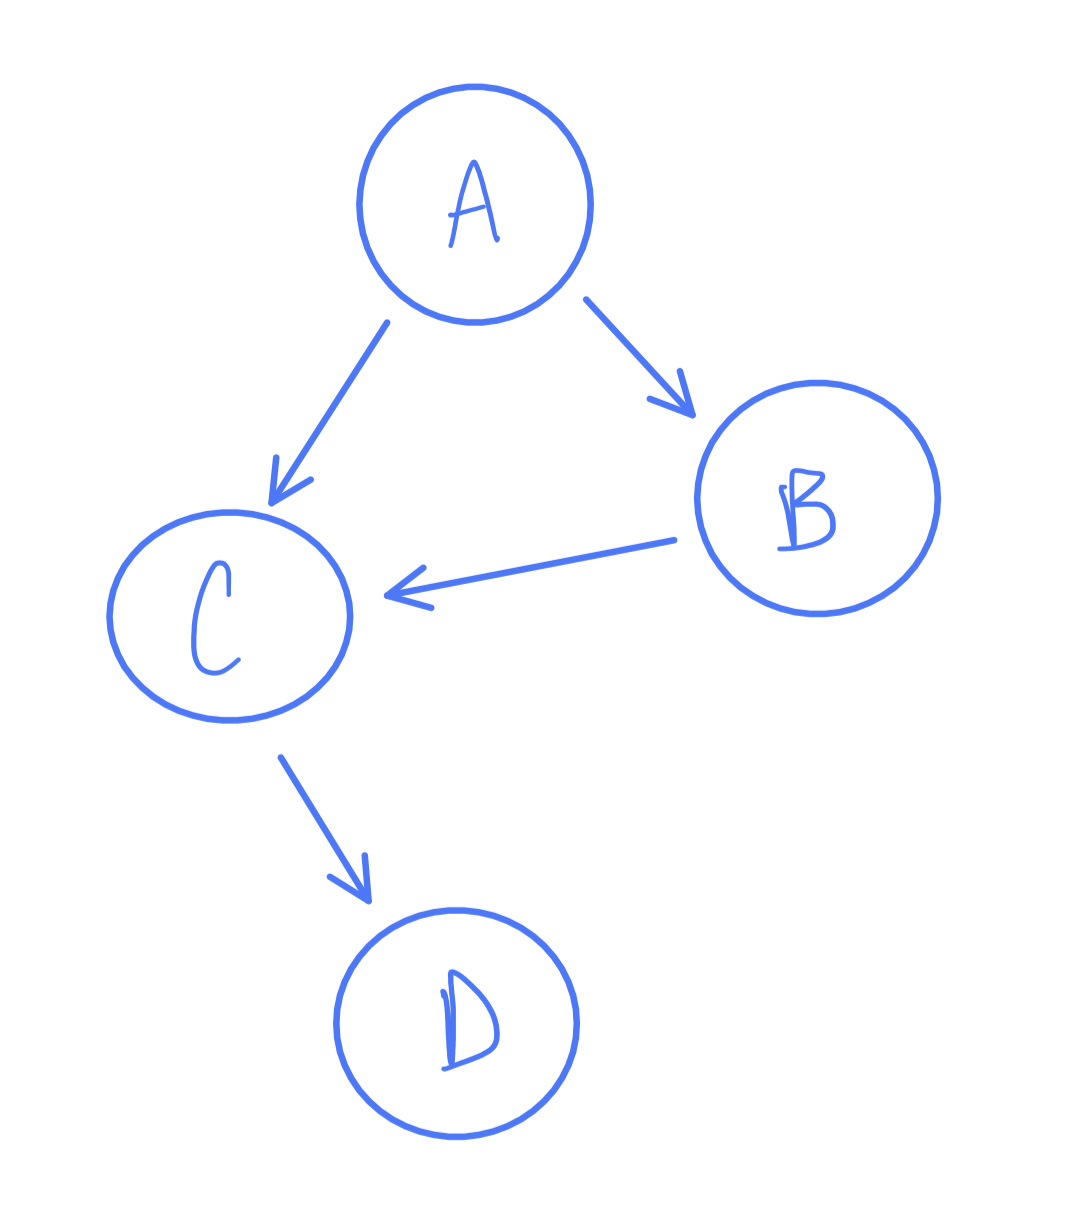
\includegraphics[width=0.6\linewidth]{"./pics/q1_graph.png"}

  \medskip
  Let the graph above represent precedence relations where $A$ has no restrictions, $B$ must come after $A$, $C$ must come after $A$ and $B$, and $D$ must come after $C$. 

  \medskip
  Consider a possible depth-first traversal of this graph starting at $A$. In the preorder list, $(X, X)$ indicates a vertex and the time it is visited beginning at zero: $(A, 0), (C, 1), (D, 2), (B, 3)$. 

  \medskip
  Sorting this by increasing preorder time yields an invalid topological sort of $A \rightarrow C \rightarrow D \rightarrow B$. This is not a valid topological sorting because $B$ must come before $C$ and here it is not.
  
\end{quote}

\item 
{\bf (7 points)}
Same as above, but we try to sort by decreasing preorder time.
\begin{quote}
  \color{purple}
  Consider the same graph as above and the same search path as above: $(A, 0), (C, 1), (D, 2), (B, 3)$.

  \medskip
  Sorting this by decreasing preorder time yields an invalid topological sort of $B \rightarrow D \rightarrow C \rightarrow A$. This is not a valid  topological sorting because $A$ must come before $B$ and $C$ but here it does not.
\end{quote}

\end{enumerate}


\item
{\bf (15 points)}
The {\em risk-free currency exchange problem} offers a risk-free way
to make money.  Suppose we have currencies $c_1,\ldots,c_n$.  (For
example, $c_1$ might be dollars, $c_2$ rubles, $c_3$ yen, etc.)  For
various pairs of distinct currencies $c_i$ and $c_j$ (but not
necessarily every pair!) there is an exchange rate $r_{i,j}$ such that
you can exchange one unit of $c_i$ for $r_{i,j}$ units of $c_j$.
(Note that even if there is an exchange rate $r_{i,j}$, so it is possible to
turn currency $i$ into currency $j$ by an exchange, the reverse might not
be true--- that is, there might
not be an exchange rate $r_{j,i}$.)  Now if, because of exchange rate
strangeness, $r_{i,j} \cdot r_{j,i} > 1$, then you can make money
simply by trading units of currency $i$ into units of currency $j$ and
back again.  (At least, if there are no exchange costs.)  This almost
never happens, but occasionally (because the updates for exchange
rates do not happen quickly enough) for very short periods of time
exchange traders can find a sequence of trades that can make risk-free
money.  That is, if there is a sequence of currencies
$c_{i_1},c_{i_2},\ldots,c_{i_k}$ such that $r_{{i_1},{i_2}} \cdot
r_{{i_2},{i_3}} \ldots \cdot r_{{i_{k-1}},{i_k}} \cdot r_{{i_k},{i_1}}
> 1$, then trading one unit of $c_{i_1}$ into $c_{i_2}$ and trading
that into $c_{i_3}$ and so on back to $c_{i_1}$ will yield a profit.

Design an efficient algorithm to detect if a risk-free currency exchange
exists.  (You need not actually find it.)

(Note: You may find the question above more accessible after the Monday (Feb. 5) lecture.)

\begin{quote}
  \color{purple}
  \textit{Note: Assertions about the Bellman Ford algorithm and Kosaraju's algorithm come from lecture notes and CLRS Ch. 22}.

  \medskip
  Let the problem be defined as above with inputs representing a directed graph as an adjacency list of currencies and their exchange rates. In this explanation, assume a currency is synonymous with a vertex and a weighted edge is parallel to $r_{i,j}$ in the question.

  \medskip
  By Lemma 1 below, a cycle of vertices $C = c_a, c_b, \dots, c_k, c_a$ such that $r_{a, b} \cdot r_{b, b + 1} \cdot \dots \cdot r_{k, a} > 1$ is equivalent to finding a negative weight cycle in a graph of the same vertices where $-\lg r_{a, b} - \lg r_{b, b + 1} - \dots - \lg r_{k, a} < 0$. The Bellman Ford algorithm detects negative-weight cycles. By Lemma 2 below, such a cycle will be in a strongly connected component (SCC). By using Kosaraju's algorithm to find every SCC and returning true if Bellman Ford detects a negative weight cycle, this problem can be solved in time $O(VE)$. The pseudocode below implements this algorithm:

  \begin{verbatim}
  fn risk_free_forex(adj: Graph as adjacency list) -> boolean:
      list of SCCs = Kosaraju's Algorithm on adj;

      for SCC as (list of vertices, list of edges) in SCCs:
          for edge in edges:
              edge.weight = -1 * lg(edge.weight);
          if Bellman Ford(vertices, edges, edges[0]) returns false: 
              return true;

      return false; 
  \end{verbatim}

\medskip 
\textbf{Correctness}:\\ 
\textit{Lemma 1}, if a cycle $c_a, c_b, \dots, c_k, c_a$ exists such that $r_{a, b} \cdot r_{b, b + 1} \cdot \dots \cdot r_{k, a} > 1$, then $-\lg r_{a, b} - \lg r_{b, b + 1} - \dots - \lg r_{k, a} < 0$: Proof by this series of algebraic manipulations: 
\begin{align*}
    && r_{a, b} \cdot r_{b, b + 1} \cdot \dots \cdot r_{k, a} > 1 && \text{Initial} && \\
    && \lg (r_{a, b} \cdot r_{b, b + 1} \cdot \dots \cdot r_{k, a}) > \lg 1 && \text{Apply log} && \\
    && \lg r_{a, b} + \lg r_{b, b + 1} + \dots + \lg r_{k, a} > 0 && \text{Log multiplication rule} && \\
    && -\lg r_{a, b} - \lg r_{b, b + 1} - \dots - \lg r_{k, a} < 0 && \text{Divide by $-1$} && \\
\end{align*} 

\medskip
\textit{Lemma 2}, if such a cycle from Lemma 1 exists in the graph, then it's an SCC: Let $C = c_a, c_b, \dots, c_k, c_a$ be the vertices of such a cycle. Let $c_m$ be any of these vertices in $C$. By definition of cycle, $c_m$ is reachable from $c_a$. By definition of cycle, $c_a$ is reachable from $c_m$. Because $c_m$ can be any vertex in $C$, every vertex in the cycle is reachable from every other vertex in the cycle, making it an SCC. 

\medskip
\textit{Proof 1}: If there's a risk free cycle $C$ as defined above, the algorithm returns true. 

\medskip
By Lemma 2, considering every SCC individually cannot change the existence of a risk-free cycle in the graph. Similarly, it makes the choice of \texttt{vertices[0]} as Bellman Ford \texttt{start} arbitrary. By Lemma 1, if such a cycle exists in any SCC, it will manifest after conversion as a negative weight loop. The Bellman Ford algorithm always returns false if a negative weight cycle exists, so it will always return false if a negative weight cycle exists in the SCC it's given. Because every SCC is considered, the algorithm will always return true if a negative weight cycle exists anywhere in the graph, thus returning true if a risk free cycle exists in the graph. 

\medskip
\textit{Proof 2}: The algorithm only returns true if there's a risk free cycle. 

\medskip
Because of the if-condition on Bellman Ford, this algorithm only returns true if a negative-weight cycle is detected in the converted graph. By the algebraic reverse of Lemma 1, such a cycle $C$ only exists when $r_{a, b} \cdot r_{b, b + 1} \cdot \dots \cdot r_{k, a} > 1$. So, the algorithm only returns true if a risk free cycle exists in the graph.  

\medskip
By the two proofs above, assert the correctness of the algorithm. 

\medskip
\textbf{Runtime}: \\ 
Let $V$ be the number of vertices and $E$ be the number of edges in the input graph. This algorithm makes the following assumptions compatible with common implementations of Kosaraju's Algorithm and the Bellman Ford algorithm: (1) Kosaraju's algorithm runs in time $O(V + E)$ given an adjacency list; (2) Kosaraju's algorithm can return a list of strongly connected components each containing a list of vertices and a list of edges without affecting its asymptotic runtime or correctness; (3) Bellman Ford takes time $O(VE)$ when given a list of vertices and a distinct list of edges. 

\medskip
Kosaraju's algorithm returns a list of length $S$ where $S$ is the number of SCCs in the graph and runs in time $O(V + E)$. Because the count of all vertices and edges in the graph is less than or equal to the count of all vertices and edges in all SCCs in the graph, assume without loss of generality that each SCC contains $O(\frac{V}{S})$ vertices and $O(\frac{E}{S})$ edges. Thus, converting the edges within each SCC takes time $O(\frac{E}{S})$ and Bellman Ford takes time $O(\frac{VE}{C})$. After $S$ iterations, the loop takes time $S \cdot (O(\frac{E}{S}) + O(\frac{VE}{S})) = O(VE) + O(E) = O(VE)$. Thus, the total algorithm runs in time $O(V + E) + O(VE) = O(VE)$. 
\end{quote}

\item %Pebbling Games.
In this problem we consider two versions of ``Pebbling Games", a class of ``solitaire'' games (played by one player). In both versions, the input to the game  includes an undirected graph $G$ with $n$ vertices and $m$ edges, and positive integer parameters $c$ and $k\le n$. At the beginning of the game, the player is given $k$ pebbles which are placed on vertices $0$, $1$, \ldots, $k-1$. At any given moment of time, the $k$ pebbles are located at some $k$ (not necessarily distinct) vertices of the graph. In each move, the player can move any pebble to a vertex $v$, provided that prior to this move, at least $c$ vertices adjacent to $v$ have a pebble. (The pebble moved does not have to be one of those that start out adjacent to $v$.)
\begin{enumerate}
    \item 
    {\bf (20 points)}
    In version 1 of the game, we have $c=k=1$ and so the unique pebble effectively moves across an edge of the graph. In this version, the player wins if there is a strategy that traverses every edge (in both directions) in exactly $2m$ moves, where $m$ is the number of edges of $G$. Give a winning strategy (i.e., an algorithm that outputs an order in which the edges are traversed) for the player for every connected graph $G$. 
    \begin{quote}
      \color{purple}
      Assume the input graph is given as an adjacency list hash map where each key is a vertex number and each value is a set of the vertex numbers adjacent to the key vertex. Further assume that undirected edges are unique (because they're in a set) and that an edge from $a$ to $b$ is represented with $b$ in the set for $a$ and $a$ in the set for $b$. Assume the output path is a list of vertices such that any two adjacent vertices represent an edge to be traversed in order from left to right.  

      \medskip
      Consider this algorithm based on DFS: Let there be a function \texttt{search} that takes the adjacency list of edges, the current vertex number, and the path list. The initial call is the full adjacency list, vertex 0, and an empty list. The search function first adds its id to the \texttt{path}. Then, while its list of adjacent edges is not empty, it pops a neighbor, removes itself from its neighbor's list, searches the neighbor, and pushes its id to the \texttt{path} again. Finally, it returns the \texttt{path} list. Here's pseudocode for such an algorithm: 

  \begin{verbatim}
  fn search(
      edges: Hash map(vertex num, neighbor set), 
      curr: vertex num, 
      path: vertex list
  ) -> vertex list:
      path.push(curr);

      while edges[curr] is not empty:
          neighbor = pop from edges[curr];
          remove curr from edges[neighbor];
          search(edges, neighbor, path);
          path.push(curr);

      return path;
  \end{verbatim}

  \textbf{Correctness}: \\
  In the proofs below, define searching an edge $(v_i, v_k)$ as calling \texttt{search} from vertex $v_i$ on a neighbor $v_k$.

  \medskip
  \textit{Lemma 1}, once an edge $(v_i, v_k)$ is searched, it is never searched again: All edges are stored in the adjacency list. The only way an edge is searched if it is selected and removed entirely from the adjacency list within the while loop. After this, it can never be found and searched again because it has been deleted.

  \medskip
  \textit{Lemma 2}, every edge is searched exactly once: By Lemma 1, an edge is not searched more than once. The input graph is connected, so every vertex is reachable from the start. The loop searches all edges neighboring the current vertex. All vertices are reachable from the start, and edges are only deleted once they've been searched. So, every vertex is reached by \texttt{search}, impliying that every edge is searched. Thus, every edge is searched once.

  \medskip
  \textit{Lemma 3}, \texttt{search} from $v_i$ to $v_k$ crosses the edge between them exactly twice: Calling search on $v_k$ from $v_i$ crosses the edge once. Because the edge is deleted, the recursive search starting at $v_i$ will not reverse search to $v_k$. Because the number of edges is finite and Lemma 2 asserts that every edge is searched once, the recursive call will eventually unwind, returning to $v_k$, crossing the edge a second time. Because the edge was previously deleted from the adjacency list, it will never be crossed again. 
      
  \medskip
  \textit{Lemma 4}, The \texttt{path} list mirrors the search path described in the lemmas above: For any vertex in any position along the search path, when the stack frame begins, its vertex id \texttt{curr} is pushed to the path. In the while loop, the recursion stack may grow, but every time it returns to the current frame, \texttt{curr} is pushed to \texttt{path} again. The \texttt{path} list is only ever mutated in this way according to the current frame's \texttt{curr}, so it must be the case that \texttt{path} mirrors the algorithm's search path. 

  \medskip 
  \textit{Proof of correctness}: If a path is returned, it visits every vertex by traversing every edge twice. By Lemmas 1 through 3 above, assert that the algorithm searches every edge in the graph exactly once, crossing every edge exactly twice, and recording its path correctly in the \texttt{path} list. By Lemma 4, assert that such a is correctly encoded in the returned path. This is the only way the returned path is generated, so the returned path must correctly identify a traversal of the graph visiting every vertex and crossing every edge twice. 

  \medskip
  If a winning strategy exists, it is returned: assert from Lemmas 1 thorugh 3 that the graph search visits every vertex once and crosses every edge twice. In doing so, the search naturally generates a winning strategy and encodes into the returned path, which, by Lemma 4, correctly encodes the search path. 

  \medskip 
  \textbf{Runtime}: \\
  Assume that list push, set pop, and set remove are constant time operations. Assert from the correctness proof that each edge is searched exactly once. So, \texttt{search} is called $m$ times where $m$ is the number of edges in the graph. If \texttt{search} is called $m$ times, it must be the case that the cumulative while loop iterations across all calls to \texttt{search} also execute on the order of $m$ times. Because all the other operations performed in \texttt{search} execute in constant time, the total complexity of calling \texttt{search} on a graph with E edges is $O(m)$. 
    \end{quote}
    \item 
    {\bf (20 points)}
    In version 2 of the game, $c$ and $k$ are arbitrary and there is a special designated target vertex $t$ such that the player wins if they can place a pebble on $t$ in any finite number of moves. Give an algorithm to determine if a given graph $G$ has a winning strategy. For full credit, your algorithm should run in time at most $O(n^{2k})$. 
    \begin{quote}
      \color{purple}
      \textit{Note: We haven't covered dynamic programming in class yet, but this was the only way I could think to solve this question. While it may not be the solution you're looking for, I believe it still should work}. 

      \medskip
      First, note that if $k == c == 1$, question $a$ applies and we know $t$ is reachable. Assume that $k$ is never less than $1$ because the pebble placement notation doesn't seem to support that. Outside of edge cases, an algorithm to solve this problem must search the graph. Consider the game as a state machine. Each vertex may have one of the $k$ pebbles on it, and pebbles can move based on the rules stated above. I propose an algorithm that DFS searches each of these states, caching previously searched states to prevent cycles and reduce time complexity. When a winning state is found, the search unwinds, returning true. Else, if every state reachable from start is searched and no winning state is found, false is returned. The algorithm below accomplishes this:

      \medskip
      Define \texttt{winnable} as a wrapper for search that catches the edge cases mentioned above and calls \texttt{search}. Define \texttt{search} as such a function: given a state $S$ representing the set of vertices with a pebble on them, return true if $t$ has a pebble on it. If the state has been searched before, return the result of the previous search. Else, for every vertex neighboring a pebble vertex in $S$, check if it's possible to move a pebble to that neighbor. If so, for every pebble that could be moved from a current vertex in $S$ to the new vertex, move that pebble and \texttt{search} the new state. If \texttt{search} returns true, return true. Else, keep searching until all states are exhausted, at which point return false. The pseudocode below implements this algorithm: 
      \newpage

    \begin{verbatim}
    fn winnable(adj: graph as adjacency list, c: int, k: int, t: int) -> bool: 
        assert k >= 1;
        if k and c are both 1:
            return true;
        dp = Hashmap(set of vertices, boolean);
        pebbles = { 0, 1, ..., k - 1 };
        dp[pebbles] = true;
        return search(adj, c, k, t, pebbles, dp);

    fn search(
        adj: graph as adjacency list,
        c: int,
        k: int,
        target: int,
        pebbles: set of vertices with pebbles on them,
        dp: Hashmap(set of vertices, boolean),
    ) -> bool: 
        if target in pebbles:
            return true;
        
        if pebbles in dp:
            return dp[pebbles];

        for v_pebble in pebbles:
            for neighbor of v_pebble:
                if neighbor in pebbles:
                    continue;

                adj_ct = 0;
                for adj of neighbor:
                    if adj in pebbles:
                        adj_ct += 1;
                if adj_ct < c:
                    continue

                for v_evict in pebbles:
                    new_pebbles = pebbles - v_evict + neighbor;
                    if search(adj, c, k, target, new_pebbles, dp) == true:
                        dp[pebbles] = true;
                        return true;

         dp[pebbles] = false;
         return false;
    \end{verbatim}
    \newpage

    \textbf{Correctness}: \\ 
    \textit{Lemma 0}, Every state reachable with fewer than $k$ pebbles is reachable with $k$ pebbles: Given any state reachable with fewer than $k$ pebbles, undo the previous state transition. Then, add pebbles to any vertex currently with a pebble until there are $k$ pebbles in the system. Because no vertices lost a pebble, the number of viable transition states has not decreased, so the state transition can be performed again. Because this applies to any transition with any nonzero number of pebbles, the claim must be true. 

    \medskip
    \textit{Lemma 0.5}, In two systems with the same number of pebbles in total, a system $A$ where each vertex with a pebble has one \textit{or more} pebbles has the same or fewer transition relations as a system $B$ where each vertex with a pebble has exactly one pebble assuming every pebble vertex in $A$ is a pebble vertex in $B$: Because both systems have the same number of pebbles, $A$ has the same or more possible transition states as $B$ because it has the same or more vertices with pebbles. This is because a non-pebble vertex is a valid transition no matter how many pebbles are on each of its neighbors as long as a neighbor has at least one pebble on it.    

    \medskip
    \textit{Lemma 1}, Only valid states are searched: A valid state is one that can be reached from the initial state by following the rules of the game. Proof by strong induction: 
    \begin{itemize}
      \item Base case: The initial state is definitionally valid.  
      \item Inductive hypothesis: Assume the claim is true for all states up to the $k$th state transition.
      \item Inductive step: At the $k + 1$ state transition, by the inductive hypothesis, the current state was reached in a valid way. At this step of iteration, if true is not returned, every pebble move to every viable neighbor vertex is considered. A pebble is only moved if the new vertex has at least $c$ neighbors with pebbles, satisfying that rule of the game. Any pebble can be moved to that vertex within the rules. In this way, a pebble is only moved if doing so generates a valid state. Thus, every state searched at this step is also a valid state. This proves the claim by induction
    \end{itemize}

    \medskip
    \textit{Lemma 2}, Every reachable state is searched until there are no remaining states to search or true is returned: At each recursive step, every valid state transition one pebble move away from the current state is searched. Because already-searched states return immediately, only new states are recursively evaluated and searched. If any winning state is found, true is returned, and the call chain unwinds as all return true. Else, the search continues via DFS until every reachable state from start is searched. At that point, there are no more states to search, and the call chain unwinds returning false. In this way, either a winning state is found and true is returned or the entire set of reachable valid states is searched until false is returned. 

    \medskip
    \textit{Proof of correctness}, If there's a way to win the game, true is returned from the algorithm: First, assert from Lemma 0 and Lemma 0.5 that any winning state that can be found by putting pebbles on the same vertices is winnable by keeping pebbles on distinct vertices. Because of this, neither the algorithm nor correctness proof attend to the case of putting multiple pebbles on the same vertex. 

    \medskip
    Considering the pseudocode, if $k == c == 1$, assert from the proof for part $a$ that every vertex can be reached and thus a winning strategy is always possible. Else, assert from Lemma 2 that every possible state reachable from the initial state is searched. If any such state has a pebble on vertex $t$, then true is returned from the algorithm. Else, if no state reachable from the initial state by the transition rules has a pebble on $t$, then false is returned. Both outcomes satisfy the rules of the game.

    \medskip
    If true is returned from the algorithm, there's a way to win the game: Assert from Lemma 1 that only valid states are searched. If \texttt{search} is called on a state and a pebble is on $t$ at that state, true is returned. Aside from that case, true is only ever returned if a recursive call returns true, so true is only ever returned if a valid state is reached with a pebble on $t$. By definition, that indicates a valid way to win the game. 

    \medskip
    By these two cases, the algorithm correctly solves the problem.

    \medskip 
    \textbf{Runtime}: \\
    First, consider the complexity of a single call to \texttt{search}. If the state has already been searched or the state is winning, the function exits in $O(1)$. Else, the pebble loop takes $O(k)$, iterating neighbors takes $O(n)$, counting pebble neighbors takes $O(n)$, iterating swap pairs takes $O(k)$, and generating a new pebble set takes $O(k)$. Within the bottom loop, expect search to be recursively called another $O(n)$ times because winning states and \texttt{dp} aren't checked until the recursive call. Thus, calling \texttt{search} on a new, non-winning state takes $O(kn(n + k(k + n))) = O(kn^2 + k^3n + kn^2)$ time, which simplifies to $O(n^2)$ because $k$ is a constant. A full search is performed on at most every possible state in the state space. Because the state space consists of $k$-sized combinations of $n$, there are $n$ choose $k$ combinations in the state space. Assert that $n$ choose $k$ is $O(n^k)$. 

    \medskip
    Because of the initial check in \texttt{winnable}, the algorithm returns true in $O(1)$ when $k == c == 1$. Else, it runs in $O(n^k \cdot n^2) = O(n^{k + 2})$. By these two cases, note that the algorithm always runs in time $O(n^{2k})$ assuming $k \geq 1$.  

    \end{quote}
    \item {\bf (0 points, optional)}\footnote{This question will not be used for grades, but try it if you're interested.
    It may be used for recommendations or TF hiring.} 
    Find an algorithm for version 2 of the game which runs in time $o(n^{2k})$---the faster, the better!
\end{enumerate} 

\item It sometimes happens that a patient who requires a kidney transplant has someone (e.g. a friend or family member) willing to donate a kidney, but the donor's kidney is incompatible with the patient for medical reasons. In such cases, pairs of a patient and donor can enter a \emph{kidney exchange}. In this exchange, patient-donor pairs $(p_i,d_i)$ may be able to donate to each other: there's a given function $c$ such that for each pair $(i,j)$ of patient-donor pairs, either $c(i,j) = 1$, meaning that $d_i$ can donate a kidney to $p_j$, or $c(i,j) = 0$, meaning that $d_i$ can't donate a kidney to $p_j$. As an example, suppose that we have five patient-donor pairs: $$(p_1,d_1), (p_2,d_2), (p_3,d_3), (p_4,d_4), (p_5,d_5).$$ Suppose also that $c(3,2) = c(3,1) = c(2,1) = c(1,3) = 1$, and that for all other inputs $c$ is 0. That is, in this example, $d_3$ can donate to $p_2$ or $p_1$, $d_2$ can donate to $p_1$, and $d_1$ can then donate to $p_3$ in the original $(p_3,d_3)$ pair. Then a set of these donations can simultaneously occur: e.g. $d_3$ gives a kidney to $p_2$, $d_2$ gives a kidney to $p_1$, and $d_1$ gives a kidney to $p_3$. (In this example, $(p_4,d_4)$ and $(p_5,d_5)$ don't participate). For every donor that donates a kidney, their respective patient must also receive a kidney, so if instead $c(1,3) = 0$, no donations could occur: $d_3$ will refuse to donate a kidney to $p_2$ because $p_3$ won't get a kidney.
\begin{enumerate}
    \item {\bf (5 points)} Give an algorithm that determines whether or not a set of donations can occur. 
      \begin{quote}
        \color{purple}
Consider this algorithm: represent the pairs as a directed graph. Each donation is an edge from donor $m$ to patient $n$. Because donations only occur when patient $m$ also has a donor, add another edge from patient $m$ to donor $m$. After all pairs are encoded this way, every donor will have edges out to a patient representing the donation, and every patient $m$ will have exactly one edge to donor $m$. After the input is encoded this way, return true if every disconnected component in the graph is a cycle. Otherwise, return false. Here's pseudocode for such an algorithm:

\newpage
  \begin{verbatim}
let STATE = unexplored or explored;

fn valid_donations(pairs: (donor m, patient n) list) -> bool:
    let (adj, states) = encode_pairs(pairs);
    for curr_vertex in states:
        if states.curr_vertex is explored:
            continue;
        if find_cycle(adj, states, curr_vertex) doesn't return Some(curr_vertex): 
            return false;
    return true;

fn encode_pairs(pairs: (donor m, patient n) list) -> (
  adjacency list, 
  HashMap(vertex id, STATE)
):
    let adjacency list adj = HashMap(vertex id, neighbor set);
    let states = HashMap(vertex id, STATE);
    for (donor m, patient n) in pairs:
        adj[donor m].add(patient n);
        adj[patient m].add(donor m);
        set states of donor m, patient n, and patient m to unexplored;
    return (adj, states);


fn find_cycle(adj, states, vertex) -> Option(vertex):
    if states.vertex is explored:
        return Some(vertex);

    states.vertex = explored;
    for neighbor in adj[vertex]:
        if is_cycle(adj, states, neighbor) returns Some(v):
            return Some(v);

    return None;
  \end{verbatim}

  \textbf{Correctness}: \\ 
  \textit{Lemma 1}, \texttt{encode\_pairs} returns an adjacency list graph such that the matching can occur only if every disconnected component is a cycle: For every (donor $m$, patient $n$) pair, an edge is added from $m$ to $n$. This encodes the possibility of $m$ donating to $n$. Simultaneously, an edge is added from patient $m$ to donor $m$, which encodes donor $m$ having permission to donate. Because the only edges in this bipartite graph from patients to donors are created using the second method stated above, there's a number of capable donors exactly equal to the number of patients. Thus, if every donor has an edge in, every donor can have an edge out. If the edges in and out across the entire graph form a cycle, then there is an alternating walk between patients and donors such that every patient is matched with a donor. If every patient does not have a donor, then not every donor has permission from a patient to donate. In this circumstance, the graph will not have a cycle because the un-donated patient and the un-permitted donor will block the cycle from completing. Thus, the returned graph is encoded such that if every disconnected component is a cycle, the matching can occur.  

  \medskip 
  \textit{Lemma 2}, If \texttt{find\_cycle} returns the vertex $v$ when called on $v$, then $v$ is the start of a cycle: \texttt{find\_cycle} performs a DFS.  During the search, each vertex that's visited is marked explored before recursing. Similarly, every searched vertex will be unvisited until a previously-visited vertex is found. At that point, the call chain unwinds, returning that vertex. A visited vertex is only found if the search loops back on itself or ventures into a cycle elsewhere (in the context of this problem). If it loops back on itself and the point at which it does so is the point where the search began, that's definitionally a cycle. There's no other way that $v$ can be returned when \texttt{find\_cycle} is initially called upon $v$, so it must be the case that \texttt{find\_cycle} returning $v$ when called on $v$ indicates a cycle. In reverse, assume for purposes of contradiction that $v$ is the start of a cycle but $v$ is not returned from \texttt{find\_cycle}. In the context of this question, vertices explored outside the current DFS are assumed to be in disjoint cycles, so that means the algorithm looped back on itself. But an algorithm looping back on itself at a place other than the start violates the formal definition of cycle. So, it must be the case that if $v$ is the start of a cycle, then $v$ is returned. 

  \medskip
  \textit{Proof of algorithm}, If the matching is valid, valid donations returns true: If the matching is valid, then \texttt{adj} is a directed graph where, for every disconnected component, there's a cycle  beginning at any member. Assert from Lemma 1 that the pairs are correctly encoded into a graph. By Lemma 1, every cycle within that graph will be detected, and the algorithm will return true if the matching is valid.

  \medskip
  If valid donations returns true, the matching is valid: Assume from Lemma 1 that input is correctly encoded. The algorithm will only return true if every call to \texttt{is\_cycle} indicates a cycle. Assert the correctness of \texttt{is\_cycle} from Lemma 2. If every disjoint component in the graph is a cycle, then the matching is valid.

  \medskip
  \textbf{Runtime}: \\ 
  Encoding the graph takes time $O(V + E)$ where $V$ is the number donors and patients and $E$ is the number of pairs. $E$ is distinct because the potentially invalid matching may have many more edges than vertices. After that, \texttt{valid\_donations} searches the graph to determine if it consists entirely of one or more disjoint cycles. For every vertex that's visited, either it's in a cycle or it's not. If it is in a cycle, then the entire cycle is marked as explored and never visited again. If it's not in a cycle, then the call returns false and the algorithm returns early, indicating an invalid matching. Thus, at most the entire graph is searched in this way via DFS, generating a search complexity of $O(V + E)$. 
      \end{quote}
    \item {\bf (20 points)} Suppose that no set of donations can occur in the previous part, but we add an altruistic donor, $d_0$. This altruistic donor is not bound to a patient, and is unconditionally willing to donate a kidney. Additionally, for each donation from $d_i$ to $p_j$, consider that there is some value $v_{ij}$ associated with that donation. Give an algorithm that returns the highest value donation sequence. For partial credit, you can consider the cases where 1) every donation has the same value or 2) donations have possibly-distinct but only positive values. 
      \begin{quote}
        \color{purple}
        Consider this algorithm: construct a graph using \texttt{encode\_pairs} from part $a$. Call the altruistic donor $d_a$. Begin a DFS from $d_a$ that considers every possible path and returns the path with the greatest value. Return that path and value. Such a search relies on properties proven below and is sped up by caching. Assume that the value of a donation is returned by an input utility function that returns a value given a donor and a patient. My algorithm runs on a modified version that only returns the value of the input function when the edge is from a donor, else it returns 0. Assume the initially-given list of pairs is not empty. Pseudocode below: 
        \begin{verbatim}
        #define empty linked list = ();

        let global cache = HashMap(vertex, (value, linked list path));
        let global visiting = empty vertex set;

        redefine function eval(edge from, edge to) -> value:
            if edge is from a patient:
                return 0;
            if edge is from a donor:
                return original value function(edge from, edge to);


        fn best_seq(
            pairs: (donor m, patient n) list,
            value: input utility function,
        ) -> (value, path):
            let (adj, _) = encode_pairs(pairs);
            adj[altruistic donor] = empty set;
            for (_, patient) in pairs:
                adj[altruistic donor].add(patient);

            let (val, list) = val_of_match(adj, altruistic donor);
            let new_matchings = condense_path(list);
            return (val, list);

        fn val_of_match(adj: adjacency list, curr: vertex) -> (value, path):
            if curr in visiting:
                return (0, ());
            if curr in cache:
                return cache[curr];

            visiting.add(curr);
            let best = (-infinity, ());
            for neighbor of adj[curr]:
                let (val, path) = val_of_match(adj, neighbor);
                let utility_of_match = val + eval(curr, neighbor);
                if utility_of_match > best_val:
                    best.value = utility_of_match;
                    best.path = curr :: path; // prepend to linked list
              visiting.remove(curr);

              if best_val is still -infinity:
                  return (0, curr :: ());
              cache[curr] = best;
              return best;

          fn condense_path(
              list: linked list of donor-patient pairs
          ) -> list of (donor m, patient n) pairs:
              let matched_pairs = [];
              while list has at least two elements: 
                  (donor, patient) = take first two from list;
                  matched_pairs.push((donor, patient));
              return matched_pairs;
        \end{verbatim}


      \medskip
        \textbf{Correctness}: \\ 
      \textit{Lemma 1}, if a matching does not begin at $d_a$, it is not viable. Assume for purposes of contradiction there's an input where no donations can occur without $d_a$, but, after adding $d_a$, there is a viable matching not beginning at $d_a$. Assert from Lemma 1 in part $a$ that the graph correctly encodes the input pairs. Because $d_a$ has no edges in, there is no way for the matching to include $d_a$. Thus, $d_a$ can be removed from the graph without changing the matching. Now, we have the input graph, but there is a valid matching. This contradicts the assumption that no donations can occur without $d_a$, so it must be the case that any valid matching on such a graph begins at $d_a$.

      \medskip
      \textit{Lemma 2}, any path beginning at $d_a$ is allowed under the rules of donation. Prove by induction on the number of unique edges from $d_a$:
      \begin{itemize}
        \item Base case: Because $d_a$ will donate no matter what, any edge from $d_a$ to a patient is permitted. 
        \item Inductive hypothesis: Any valid path $k$ edges from $d_a$ is permitted.  
        \item Inductive step: The $k + 1$ edge could come from either a patient or a donor. If the edge comes from a patient, that means the patient was donated to. Because the patient was donated to, their donor is free to donate. Because the patient's only edge is to their donor, this edge is permitted. If the edge comes from a donor, because $d_a$'s initial edge was to a patient, the alternating walk of the graph implies that the current donor's patient was donated to. When this is the case, the donor is free to donate to anyone they have an edge to. In either case, any edge coming from the current vertex is permitted. By induction, this proves the claim. 
      \end{itemize}

      \medskip
      \textit{Lemma 2.5}, if \texttt{val\_of\_match} returns optimal results, the path list correctly reflects the optimal matching. For every neighbor that's searched, the path is chosen that optimizes the value of the match. Assuming the subproblem returns a correctly constructed path, curr adds itself to the front of the path, which extends the path in a valid way for the current problem. Because the operation prepends to the list, any cached results that might point to nodes later in the list are still valid because the list is only ever mutated by extending the head. 

      \medskip
      \textit{Lemma 3}, if initially called from $d_a$, \texttt{val\_of\_match} returns the highest valued unique path from its given vertex. Assert from Lemmmas $1$ and $2$ that every path of unique edges is viable. Prove by induction on the DFS call stack: 
      \begin{itemize}
        \item Base case 1: The search is at a sink when it is sent to a vertex that has already been visited. In that case, it returns 0 and an empty path because a highest value from this position is nonexistent.
        \item Base case 2: The search is also at a sink when it is sent to a vertex with no out-edges. In that case, the search returns that no more value could be found from that vertex with an empty value and itself in the path. Both base cases return the best possible value from that vertex, which is 0.
        \item Inductive hypotheses: assume every recursive call returns the highest-valued unique path from the vertex it's called upon. 
        \textit Inductive step: If the given vertex is not a base case, it considers all outbound edges. By the inductive hypothesis, all recursive calls return the best possible value and path from that vertex. Thus, among all best possible paths to take, the edge with the highest value is chosen, updated, and returned. In this way, the current frame of \texttt{val\_of\_match} also returns the highest valued unique path. Assert from lemma 2.5 that the linked list properly encodes this path. This proves the claim inductively.
      \end{itemize}

      \medskip
      \textit{Lemma 4}, if an input path to \texttt{condensed\_path} is valid, the output pairs are also valid. Because the donation graph is bipartite, any valid path will alternate between donors and patients. A pairing is specified as a donor to a patient. Because the path must begin with the donor $d_a$ by Lemma 1, \texttt{condensed\_path} returns a list of (donor, patient) tuples in the order of their search path. Thus, if the search path represents a valid sequence of donations, the pairs returned from \texttt{condensed\_path} are valid. There is an edge case in which an additional donor appears at the end of the path with nobody to donate to, but this is addressed by the while loop exiting when there are only zero or one elements left in the list. Because \texttt{condensed\_path} doesn't add pairs to the returned list for any other reason, all output paths must be valid given valid input paths.  

      \medskip
      \textit{Proof of correctness}, if there is a highest value matching, it is returned. Assert from Lemma 1 in part $a$ that the input pairs are encoded into a valid graph. The altruistic donor is also introduced with an edge to every patient. Assert from Lemmas 1 and 2 that a maximum matching must begin from this donor. The updated \texttt{eval} function returns $0$ on edges unexpected by the input utility function, so the highest-value path still accomodates edges from patients back to donors. Assert from Lemma 3 that the search is a sequence of optimal subproblems, where each subproblem is solved correctly and cached, meaning that the result from the initial call must represent a maximum-value path through the graph. Assert the correctness of path decoding from Lemma 4. Thus, if a highest-value matching exists, it is found by the optimizing DFS, and the path of such a search is found, decoded, and returned. 
      
      \medskip
      If a matching is returned, it is the highest-value valid matching possible. Assert from Lemmas 1 and 2 that the path searched by \texttt{best\_seq} is valid, and assert from Lemma 3 that \texttt{val\_of\_match} returns a unique, optimal path. There is no other way a path is generated and returned. Thus, any list of pairs returned from \texttt{best\_seq} is the highest-valued matching supported by the graph.

      \medskip
      \textbf{Runtime}: \\ 
      The input graph may have any number of edge-pairs for its vertices, so constructing the initial graph takes time $O(V + E)$ where $V$ is the number of patients and $E$ is the number of pair assignments. Adding edges for $d_a$ also takes time linear in the number of patients. 

      \medskip
      Consider the complexity of a single call to \texttt{val\_of\_match}: Assume checking and mutating the the set and cache take constant time. Prepending to the path linked list also takes constant time. The recursive search runs in time linear to the number of edges a node has. 

      \medskip
      Because of the visited set, a single DFS searches at-most the entire graph and takes time $O(V + E)$. After such a search, however, the optimal sub-results of searching from any node in the graph are cached, making every subsequent call to search $O(1)$. Thus, the graph is searched in its entirety only once, making the total cost of \texttt{val\_of\_match} that of exploring and caching the entire state space, $O(V  + E)$. Because list decoding also takes time linear in the number of vertices in the graph, the total runtime of this algorithm is $O(V + E)$.
      \end{quote}
\end{enumerate}
    

\item Tony Stark has been thinking about how he can be more effective as Iron-Man and he's finally figured it out: two Iron-Men! He has two Iron-Man suits and he can control each remotely. Unfortunately, he's been having trouble getting the technology exactly right, so every time he makes a move in one suit, the other suit follows with a different move. Precisely, if Iron-Man 1 moves right, Iron-Man 2 moves up; if IM1 moves left, IM2 moves down; if IM1 moves up, IM2 moves left; and if IM1 moves down, then IM2 moves right. To slow him down, Thanos dropped one suit in Los Angeles and the other in Dallas. Tony needs your help getting both his suits back to Stark Industries in New York.
Assume that the United States can be modeled as an $n$ by $n$ grid, as below.

\begin{figure}[H]
    \centering
    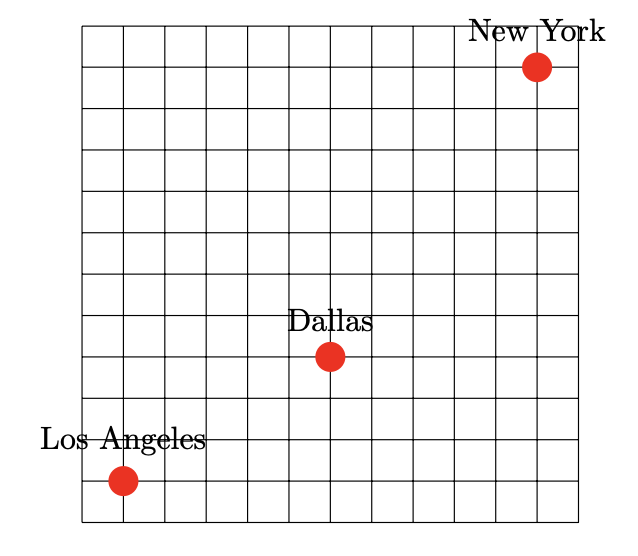
\includegraphics[width=0.4\textwidth]{tonystarkgrid.png}
    \label{fig:grid}
\end{figure}

If an Iron-Man tries to move off the grid or into an obstacle, it merely stays in place. Additionally, each step has a cost that depends on the robot's location. For example, moving left from $(0,1)$ might cost 1 fuel but moving left from $(10,15)$ might require jumping over someone's backyard pool and thus might cost 3 fuels. Once a robot reaches Stark Industries, it powers down and costs 0 fuels even as its counterpart continues to move. You are given the positions of Los Angeles $\left(x_{\ell}, y_{\ell}\right)$, Dallas $\left(x_d, y_d\right)$, and New York $\left(x_{n y}, y_{n y}\right)$, the positions of all obstacles $\left(x_{o_i}, y_{o_i}\right)$, and the cost of every possible move from every possible location.
    
\begin{enumerate}
    \item {\bf (10 points)} Give and explain an asymptotic upper bound on how many possible positions there are for the pair of Iron-Men, and explain why no better asymptotic upper bound is possible.
      \begin{quote}
        \color{purple}
        Because of obstructions and borders, IM1 and IM2 can reposition themselves relative to each other. Their relative positions are thus able to traverse the state space somewhat freely. Because of this, given enough moves, IM1 and IM2 must be capable of traversing on the order of their entire state space, yielding an upper bound of $O(n^4)$ possible positions.

        \medskip 
        This is also a lower bound. On any given n x n graph, there may exist obstructions such that IM1 can back IM2 into a corner, reposition it, and release IM2 back to freely traverse the graph 
via its relation to IM1 (and vice versa). IM1 can roam the graph as it pleases given borders and obstructions, so obstructions ensure that the state space is $\Omega(n^4)$. Simultaneously, even if, for example, 99 percent of the graph is covered by obstructions, that's still just a scalar in relation to n, so obstructions also cannot reduce the asymptotic size of the graph state space.
      \end{quote}
    \item {\bf (20 points)} Give an algorithm to find the cheapest sequence of $\{\mathrm{L}, \mathrm{R}, \mathrm{U}, \mathrm{D}\}$ moves (that is, the one that requires you to buy the smallest amount of robot fuel) that will bring both Iron-Men home to New York.
Hint: Try to represent the position of the two Iron-Men as a single vertex in some graph. For full credit, it suffices to find an $O\left(n^8\right)$ algorithm, but an $O\left(n^4 \log n\right)$ algorithm may be eligible for an exceptional score.
\begin{quote}
  \color{purple}
  Consider this algorithm: given $n$, positions, obstacles, and a cost function, construct a 4-dimensional graph where keys $(x_1, y_1, x_2, y_2)$ correspond to IM1 and IM2's positions respectively. Iterate for each of those positional dimensions and consider the possible state transitions either of the two suits could initiate. This needs to examine up, down, left, and right options in addition to borders and obstacles. The two suits might generate duplicate edges, so graph edges must be maintained in a set. 

  \medskip 
  Assume that fuel cost is always nonnegative, and define an updated cost function to return the cost of moving both suits on the 4d graph from the cost of moving one suit on the 2d graph. Run Djikstra's algorithm on the graph from the 4d coordinate placing IM1 in LA and IM2 in Dallas. From what's found, decode the path into LRUD directions and return the instructions along with the cost. Pseudocode below. Note that ".." before a data type destructures it: 

\begin{Verbatim}[xleftmargin=-6em]
type 4d coord = (IM1 x, IM1 y, IM2 x, IM2 y);

fn cheapest_seq(
    pos_la: (x, y) coord,
    pos_dallas: (x, y) coord,
    pos_ny: (x, y) coord,
    obstacles: (x, y) coord list,
    cost_fn: function mapping edges to costs,
    n: int
) -> cheapest:
    
   let graph = HashMap(4d coord, set of 4d coords):

   let updated_cost_fn = function(v_from: 4d coord, v_to: 4d coord) -> cost {
        return cost_fn(v_from.IM1, v_to.IM1) + cost_fn(f_from.IM2, v_to.IM2);
   }
    
    for IM1_row in n:
        for IM1_col in n:
            for IM2_row in n:
                for IM2_col in n:
                    let key = (IM1_row, IM1_col, IM2_row, IM2_col); 
                    for direction of up, down, left, right:
                        for suit of IM1, IM2:    
                            if suit cannot move in direction:
                                continue;
                            let other_new_pos = where other goes given suit's move;
                            let (IM1_new_pos, IM2_new_pos) = label positions of suits;
                            graph[key].add(..IM1_new_pos, ..IM2_new_pos);
    
    let start = (..pos_la, ..pos_dallas);
    let distances, paths = Djikstra(graph, updated_cost_fn, start);

    let end = (..pos_ny, ..pos_ny);
    let min_cost = distances[end];
    let moves = empty linked list;
    for move beginning at paths[end];
        let direction = decode move into direction;
        direction :: moves; // prepend to linked list

    return moves, min_cost;
  \end{Verbatim}
  
  \textbf{Correctness}:\\ 
  \textit{Lemma 1}, the set of reachable states is equal in the input and constructed graphs: Let P1/P2 be any two arbitrarily-chosen positions for the two iron men. If IM1 can move in a direction $x$, IM2 is either moved deterministically in another direction or it's blocked by a border or obstruction and vice versa. Thus, in the 2d graph, the reachable states from P1/P2 are the directions IM1 can move and the location that moves IM2 and vice versa. This is mirrored in the algorithm constructing the 4d graph, which considers each direction for each suit for each position and the edges that generates. New edges may be duplicate, but the adjacency list's edge set guarantees duplicates are filtered out. Because all the moves possible in the 2d graph are added to the 4d graph, it must be the case that any possible move in the 2d graph is encoded in its 4d counterpart. Similarly, because no other edges are added to the 4d graph, it must be the case that any move possible in the 4d graph is possible in the 2d graph.

  \medskip
  \textit{Lemma 2}, the cost of a path is the same between the 2d and 4d graphs: Prove this claim by strong induction on the cost of a path for two suits starting at positions $(x_1, y_1), (x_2, y_2)$ in the 2d graph and position $(x_1, y_1, x_2, y_2)$ in the 4d graph. Assert from Lemma 1 that any path in one version of the graph is possible in its counterpart graph.
  \begin{itemize}
    \item Base case: Initially, because no edges have been crossed, no costs have been accumulated. The path cost for both graph paths is 0.
    \item Inductive hypothesis: Assume the iron men have followed identical paths and that the costs of such paths after $k$ moves are equal. For example, for their respective graphs at move $m$ where $0 \leq m \leq k$, every $(x_{1, m}, y_{1, m}), (x_{2, m}, x_{2, m})$ coordinate is equal to every $(x_{1, m}, y_{1, m}, x_{2, m}, x_{2, m})$ coord and the costs of such paths are identical.
    \item Inductive step: At move $k + 1$, assert from Lemma 1 that IM1 and IM2 have the same set of possible moves across the two graphs. The cost of moving on the 2d graph is the cost of moving IM1 from coord $(x_{1, k}, y_{1, k})$ to $(x_{1, k + 1}, y_{1, k + 1})$ plus the cost of moving IM2 the same. By the definition of \texttt{updated\_cost\_fn}, the cost of moving the 4d coordinate with the same moves is identical. Let such a cost be $c$. Thus, the total cost is the path sum, assumed by the inductive hypothesis to be equal, plus $c$, which makes the cost of paths from 0 to $k + 1$ equal for both. This proves the claim inductively. 
  \end{itemize}

\medskip
\textit{Proof of correctness}: \\ 
If a lowest-cost path exists, the algorithm returns it: Assert from Lemma 1 that the 2d graph is properly translated into the 4d graph, and assert from Lemma 2 that path costs are the same between the two graphs. Thus, if a lowest-cost path exists in the 2d graph, the same path also exists in the 4d graph. From the correct encoding, assert the correctness of Djikstra's algorithm to find and return the shortest path from the start positions to where both suits end in New York. This assumes fuel cost is always nonnegative. Once costs and paths are returned, the path is decoded into {L, R, U, D} directions and returned along with the cost. The existence of a shorter path would contradict the correctness of Djikstra's algorithm given the correct graph encoding, so it must be the case that, if a lowest-cost path exists, it is returned.

\medskip
If the algorithm returns something, it's a lowest-cost path: Again assert the correctness of graph translation and path cost encoding from Lemmas 1 and 2. The encoded graph is processed by Djikstra's algorithm, and paths are returned. By decoding and returning the path from New York to the start positions, the algorithm is returning the path found by Djikstra's algorithm for such a route or nothing if it doesn't exist. Because Djikstra's algorithm is correct and my algorithm returns the path returned from Djikstra's algorithm, the path returned from my algorithm must be a shortest path if such a path exists.

\medskip
\textbf{Runtime}: \\ 
Begin with the observation that both the 2d and 4d graphs have a constant number of edges relative to $n$, the size of the input graph. So, any runtime expressible in terms of vertices and edges is just as correctly expressed in terms of vertices.

\medskip
While there's much constant-time conditional logic in the bottom of the graph construction loop, constructing the 4d graph ultimately takes time $O(n^4)$. After the graph is constructed, Djikstra's algorithm is run on it. Assume use of a Fibonacci heap. With $n^4$ vertices and $O(n^4)$ edges, that adds an additional $O(n^4 log n^4 + n^4) = O(n^4 log n)$ because the log exponent is absorbed as a scalar. Assume in the worst case, decoding the path requires another $O(n^4)$ steps. This yields an asymptotic
time complexity of $O(n^4 + n^4 log n + n^4)$, which simplifies to $O(n^4 log n)$.
\end{quote}
\end{enumerate}

(Note: You may find the question above more accessible after the Monday (Feb. 5) lecture.)

\item {\bf (0 points, optional)} This problem is based on the $2 \mathrm{SAT}$ problem. The input to $2 \mathrm{SAT}$ is a logical expression of a specific form: it is the conjunction (AND) of a set of clauses, where each clause is the disjunction (OR) of two literals. (A literal is either a Boolean variable or the negation of a Boolean variable.) For example, the following expression is an instance of 2SAT:
$$
\left(x_1 \vee \overline{x_2}\right) \wedge\left(\overline{x_1} \vee \overline{x_3}\right) \wedge\left(x_1 \vee x_2\right) \wedge\left(x_4 \vee \overline{x_3}\right) \wedge\left(x_4 \vee \overline{x_1}\right)
$$

A satisfying assignment to an instance of a 2SAT formula is an assignment of the variables to the values $\mathrm{T}$ (true) and $\mathrm{F}$ (false) so that all the clauses are satisfied- that is, there is at least one true literal in each clause. For example, the assignment $x_1=T, x_2=F, x_3=F, x_4=T$ satisfies the 2SAT formula above.

Derive an algorithm that either finds a satisfying assignment to a 2SAT formula, or returns that no satisfying assignment exists. Carefully give a complete description of the entire algorithm and the running time.

(Hint: Reduce to an appropriate problem. It may help to consider the following directed graph, given a formula $I$ in 2SAT: the nodes of the graph are all the variables appearing in $I$, and their negations. For each clause $(\alpha \vee \beta)$ in $I$, we add a directed edge from $\bar{\alpha}$ to $\beta$ and a second directed edge from $\bar{\beta}$ to $\alpha$. How can this be interpreted?)


\end{enumerate}



\end{document}
